\documentclass[12pt]{article}
\usepackage{natbib}
\usepackage{hyperref}
\usepackage[french]{babel}
\usepackage[utf8x]{inputenc}
\usepackage{lipsum}
\usepackage{amsmath}
\usepackage{graphicx}
\usepackage[final]{pdfpages}
\usepackage[T1]{fontenc}
%\usepackage[colorinlistoftodos]{todonotes}
\usepackage{xcolor}
\usepackage[nottoc,numbib]{tocbibind}% Para que la bibliografia salga en el table of contents
\colorlet{Mycolor1}{green!10!orange!90!}
\usepackage{subfigure}
\sloppy
\definecolor{lightgray}{gray}{0.5}
\setlength{\parindent}{0pt}
\setlength{\parskip}{1em}

\bibliographystyle{abbrv}

\begin{document}
\title{Rapport Stage}
\author{CHIRINO CAICEDO Melet}
\begin{titlepage}

\newcommand{\HRule}{\rule{\linewidth}{0.5mm}} % Defines a new command for the horizontal lines, change thickness here

\center % Center everything on the page
 
%----------------------------------------------------------------------------------------
%	HEADING SECTIONS
%----------------------------------------------------------------------------------------

\textsc{\LARGE Université Toulouse III}\\[0.5cm] % Name of your university/college
\textsc{\Large Paul Sabatier}\\[1.0cm] % Major heading such as course name
\textsc{\large Rapport du stage 2020/2021}\\[0.5cm] % Minor heading such as course title

%----------------------------------------------------------------------------------------
%	TITLE SECTION
%----------------------------------------------------------------------------------------

\HRule \\[0.4cm]
{ \huge \bfseries Projet Linky4Teens}\\[0.4cm] % Title of your document
\HRule \\[1.5cm]
 
%----------------------------------------------------------------------------------------
%	AUTHOR SECTION
%----------------------------------------------------------------------------------------

% \begin{minipage}{0.4\textwidth}
% \begin{flushleft} \large
% \markboth{Pojet en \LaTeX}
% \emph{Auteurs:}\\
% \textsc{CHIRINO} Melet \\ % Your name
% %\textsc{RIBEIRO} Bruno % Your name
% \end{flushleft}
% \end{minipage}
% ~
% \begin{minipage}{0.5\textwidth}
% \begin{flushright} \large
% \emph{Tuteur:} \\
% \textsc{RIVIERE} Nicolas  \\% Supervisor's Name
% \textsc{LABIT} Yann% Supervisor's Name
% \end{flushright}
% \end{minipage}\\[2cm]

 % If you don't want a supervisor, uncomment the two lines below and remove the section above
\Large \emph{Author:}\\
\textsc{CHIRINO CAICEDO} Melet David \\[2cm] % Your name

%----------------------------------------------------------------------------------------
%	DATE SECTION
%----------------------------------------------------------------------------------------

{\large \today}\\[2cm] % Date, change the \today to a set date if you want to be precise

%----------------------------------------------------------------------------------------
%	LOGO SECTION
%----------------------------------------------------------------------------------------


\includegraphics[width=6in]{img/Logo_UT3.jpg}\\[2cm] % Include a department/university logo - this will require the graphicx package
 
%----------------------------------------------------------------------------------------

\vfill % Fill the rest of the page with whitespace

\end{titlepage}

%\{Contents}
\tableofcontents

\newpage

%-------------------------- * Introduccion * --------------------------------

\section{Introduction}
%Aqui explico de que se trata el proyecto y lo que habiamos hecho antes como TER
Linky4Teens est un projet qui cherche \`a amelriorer le performance des jeunes athletes avec la technologie et l'electronique. Ce projet est men\'e a bien avec le profeseur Yann LABIT et le club sportif Balma, image \ref{img:LogoBalma}.
% El proyecto linky4teens es un proyecto que busca desarrollar prototipos que ayuden a mejorar el desempenho en atletas jovenes llevado por el club Balma y el Profesor Yann LABIT. El proyecto busca crear dispositivos para revisar el desempenho de los atletas y trabajar sobre los errores que se esten cometiendo. 

\begin{figure}[!htb]
\centering
\includegraphics[width=0.2\textwidth]{img/LogoBalma.png}
\caption{Club Balma}
\label{img:LogoBalma}
\end{figure}

Ce projet a commenc\'e comme un projet TER dans lequel j'ai travaill\'e dans le developpemment d'un temoin intelligent connect\'e. En tant que stagiaire, j'ai repris le developpement du temoin intelligent connect\'e et aussi un starting block developp\'e par des autres \'etudiants pour un projet TER paralelle.
% Yo estaba encargado de seguir el desarrollo de dos prototipos desarrollados en proyectos anteriores como proyectos de TER:
% \begin{itemize}
%     \item Temoin de relevos inteligente (desarrollado por mi un grupo de amigos)
%     \item Starting block
% \end{itemize}
% Estos proyectos al estar financiados por estudiantes estaban bien pero necesitaban mejoras y mucha robustez para funcionar como producto funcional.

%-------------------------- * Descripcion * --------------------------------

\section{Bref description du systeme}
% Aqui vas a mostrar unos cuantos diagramitas UML para explicar como funcionan las cosas dentro tus chocoros
En fin du projet TER le projet avait deux prototypes utilis\'ees
pour deux disciplines d'athletisme differents : Course de 
relais et un starting block.

\begin{itemize}
	\item - Le temoin a \'et\'e con\c cu pour la course de relais. Le temoin stocke
	des donn\'ees comme la vitesse et la  position vertical pour
	savoir des details lorsqu'ils font le relai.
	En plus, le temoin capte aussi si le relais est fait 
	dans la zone de relais. Apr\`es le temoin est connect\'e \`a un
	ordinateur pour voir l'information de la course et faires des
	courves pour une analise complet. 

	\item - Le starting block stocke l'information de deux capteurs de force
	plac\'es en-dessous des pieds des athletes pour savoir la force utilis\'ee
	en d\'emarrant la course. Cette information est visible
	gr\^ace \`a une courve montr\'ee a travers d'un smartphone.
\end{itemize}

%-------------------------- * Objetivos * --------------------------------

\section{Objectifs}
% Les objectifs pour le debut du projet etaient rendre les prototypes plus robustes pour une utilisation ulterieur.
% Los objetivos de stage eran rendre plus robuste los prototipos ya existentes y/o los sistemas creados.
\begin{itemize}
	\item Ameliorer le dock pour et rendre plus facile son
	utilisation car en fin du projet TER \'etait un 
	peu delicat et compliqu\'e \`a utliser.
	\item Ameliorer l'interface visuel (GUI en anglais).
	\item Rendre les temoins plus robustes et stocker plus
	d'information dedans.
	\item Rendre plus robuste le prototype du starting block
	et l'integrer \`a l'interface d\'ej\`a developp\'e.
\end{itemize}
\section{Ameliorations propos\'ees}
\begin{itemize}
    % \item Dock: utilisar una raspberry pi como dock porque esta puede usar conexion wifi direct a cualquier dispositivo que pueda acceder a internet sin necesidad de instalar porgramas o aplicaciones. 
	\item Utiliser une raspberry pi comme dock parce
	qu'elle peut se connecter a tous les appareils via
	WiFi direct pour eviter d'installer l'interface 
	dans tous les ordinateurs du club. En plus, la
	raspbery peut stocker une base de donn\'ees avec
	l'information de tous les coachs et les athletes.


    % \item Temoin: el temoin estaba soldado en una pcb universal y era muy endeble, habia que volverlo mas robusto y, el punto mas importante, no guardaba suficiente informacion, por lo tanto las mediciones eran medio jopos. Ademas el sistema de barreras IR era poco robusto. Todo eso debia mejorarlo.
	% \item Faire une pcb \`a l'aide d'un CAO pour ajouter
	% plus de compossants et rendre la partie electronique
	% plus robuste. En plus, ajouter des composants pour 
	% une utilisation plus confortable chez les athletes.
	\item Ameliorer le temoin de relais pour capter plus d'information
	et pour rendre plus robuste.
    % \item Interfaz: la interfaz utilisaba un deploy de django (un framework web escrito en python porque? porque yo lo se usar, asi de simple). Pero estaba muy simple por propias limitaciones del sistema pero con mas financiacion se podia mejorar todo.
	\item Créer une base de donn\'ees dans l'interface de tous les acteurs
	su club Balma pour avoir une tra\c cabilit\'e de la
	performance des athletes. 
	\item Établir une communication entre le starting
	block et l'interface pour manipuler les donn\'ees.
	\item Rendre l'interface multiplataforme.


    % \item Starting block: conectarlo por wifi a la interfaz para que se pueda mejar desde ahi de manera practica y sencilla. A peticion del club una base de datos no quedaria nada mal para organizar la informacion.
\end{itemize}

%-------------------------- * Obligaciones administrativas * --------------------------------
\section{Devoirs Administratives}
% Al ser un proyecto financiado por la fac tenia ciertas obligaciones administrativas como enviarle poticiones al tecnincien encharge jerome raybayrol para hacer los debis y pedir los componenetes. Ademas se me suministraron herramientas como un osciloscopio y un taladro para poder trabajar a distancia (tu sabes esto de la situacion del mundo y tales)
Vu que c'etait un projet sporsoris\'e par l'universit\'e, j'\'etais oblig\'e de me
comuniquer avec le technicien pour commander des composants et pour utiliser les
outils de l'universit\'e. Vu les conditions sanitaires j'ai du aussi pr\^eter 
des outils pour avancer en teletravail.

%-------------------------- * Obligaciones Tecnicas * --------------------------------
\section{Devoirs Techniques}
% Este proyecto tuvo muchas cosas desarrolladas en computador y muchisima programacion. Sin embargo tambie tuve mucha accion en el fablab de la fac para fabricar piezas en la impresora 3d, la cortadora laser y la maquina cnc para hacer unos circuitos.
% Ce projet a eu beaucoup des choses develop\'es en CAO et pas mal de programation, mais aussi 
% le travail sur le hardware a \'et\'e fait chez CampuFab avec la decoupe laser, la machine CNC,
% les imprimantes 3D et ses outils en general comme les perceuses, les pinces, etc.
\begin{par}
	Dans ce projet j'ai dû utiliser des logiciels de CAO,
	logiciels et outils de fabrication, outils de gestion
	de version du code et des outils pour gerer le projet
	et la documentation du même. Je n'étais pas obligé 
	d'utiliser des certains logiciels mais le technicien m'a
	conseillé d'utiliser des logiciels open source ou gratuit
	si jamais l'université n'avais pas la license.
\end{par}
\subsection{Logiciels de CAO}

\begin{par}
	Comme logiciel de CAO electronique j'ai choisi Eagle parce qu'il
	est open source et je l'avais utilisé precedement. D'ailleurs
	le technicien du service electronique de l'université utilise
	Eagle aussi donc nous pouvons eviter des problèmes de compatibilité.
	Sur la figure \ref{img:eagle_all} vour trouverez des images.
\end{par}
\begin{figure}[!htb]
	\centering
	\subfigure[Schema du circuit]{\includegraphics [height=2in]{img/EagleSchema.png}
	\label{img:eagle:schema}}
	\subfigure[PCB du circuit]{\includegraphics [height=2in]{img/EagleBoard.png}
	\label{img:eagle:board}}
	\caption{Captures d'Eagle}
	\label{img:eagle_all}
\end{figure}

\begin{par}
	Pour la fabrication des circuits avec une machine CNC j'ai
	utilisé FlatCAM (image \ref{img:FlatCam}) parce qu'il est gratuit et la sa documentation
	est facile a trouver en ligne.
\end{par}
% Los logiciel de CAO son muy importantes, para fabricar los circuitos, simularlos y disenhar su fabricacion. Como logiciel utilise Eagle (tambien porque era el que sabia usar). 
% Para los dispositivos 3D utilise la plataforma online OnShape la cual es gratuita y tambien permita compartir los disenhos en 3D con todos los participantes del proyecto (si solo hubiera mas gente) y tambien gestionar las versiones. sur la bibliographie vous trouverez le repo avec les fichiers
\begin{par}
	Pour la conception mecanique j'ai utilis\'e la plateforme \href{https://www.onshape.com/}{OnShape}
	parce qu'elle est gratuit et permet de partager les conceptions au fur et a mesure du developpement.
	quelques captures d'ecran sur la figure \ref{img:onshape_all}.
\end{par}
\begin{figure}[!htb]
	\centering
	\subfigure[Conception de la Barriere IR]{\includegraphics [height=2in]{img/OnShapeBarriere.png}
	\label{img:onshape:barriere}}
	\subfigure[Boite du starting block]{\includegraphics [height=2in]{img/OnShapeSB.png}
	\label{img:onshape:sb}}
	\subfigure[Conception mecanique du temoin]{\includegraphics [width=2.7in]{img/OnShapeTemoin.png}
	\label{img:onshape:temoin}}
	\caption{OnShape}
	\label{img:onshape_all}
\end{figure}
`%Aqui coloca imagenes del repo asi como la url del repo
\subsection{Service electronique de Paul Sabatier}
% Para fabricar circuitos alguien me informo que puedo acceder al servicio de fabricacion electronica de la universidad, tuve que ponerme en contacto con el senhor guillaume Maffre quien me gui por el proceso. A mediados del mes de mayo cambiaron el proceso de metalizacion y al parecer no era tan efectivo como el anterior porque varios circuitos no tenian bien la metalizacion, es el proceso que conecta la capa de arriba con la de abajo. Ademas este proceso tomaba de 3 dias a una semana dependiando de la complejidad del pcb. Por lo cual decidi no usar este servicio a menos que fuera estrictamente necesario.
\begin{par}
	L'universit\'e a une service de fabrication des PCBs
	lequel j'ai utilis\'e parce qu'il y a des 
	PCBs qui avaient besoin de double couche de cuivre. 
	Au millieu du mois de Mai le service electronique a 
	chang\'e le procesus de metalisation qui n'est pas
	ma\^itriss\'e au fond et alors plusieurs 
	circuits fabriqu\'es par eux n'ont pas eu la fiabilit\'e
	attendue. En plus, ce methode prenait vers une semaine
	d'attente de ma part donc j'ai decid\'e de ne utiliser
	ce service que si besoin stricte.
\end{par}

\subsection{Fabrication chez CampusFab}
% El hecho de trabajar con hardware requiere muchas herramientas y espacio para trabajar, lo cual no tengo en casa. GraciajaDios la fac cuenta con el fablab del cual soy abone y me puedo en servir de todas sus herramientas y maquinas.
\begin{par}
	Pour travailler le hardware j'ai choisi CampuFab parce que j'\'etais d\'ej\`a
	familiaris\'e avec les outils qui s'y trouvent et parce qu'ils ont des horarires
	flexibles. Dans l'image \ref{img:CampusFab}
	et \ref{img:CircuitsCNCd}
\end{par}

% La primera herramienta que use fue la maquina cnc para fabricar unas pcb pequenhas. Este proceso lo hice con la ayuda del logiciel flatCAM y un simulador de maquinas cnc porque con la situacion sanitaria tenia que priorizar al maximo el teletrabajo.
\begin{figure}[!htb]
	\centering
	\subfigure[FlatCAM]{\includegraphics[width=0.65\textwidth]{img/FlatCAM.png}
	\label{img:FlatCam}}
	\subfigure[Machine CNC]{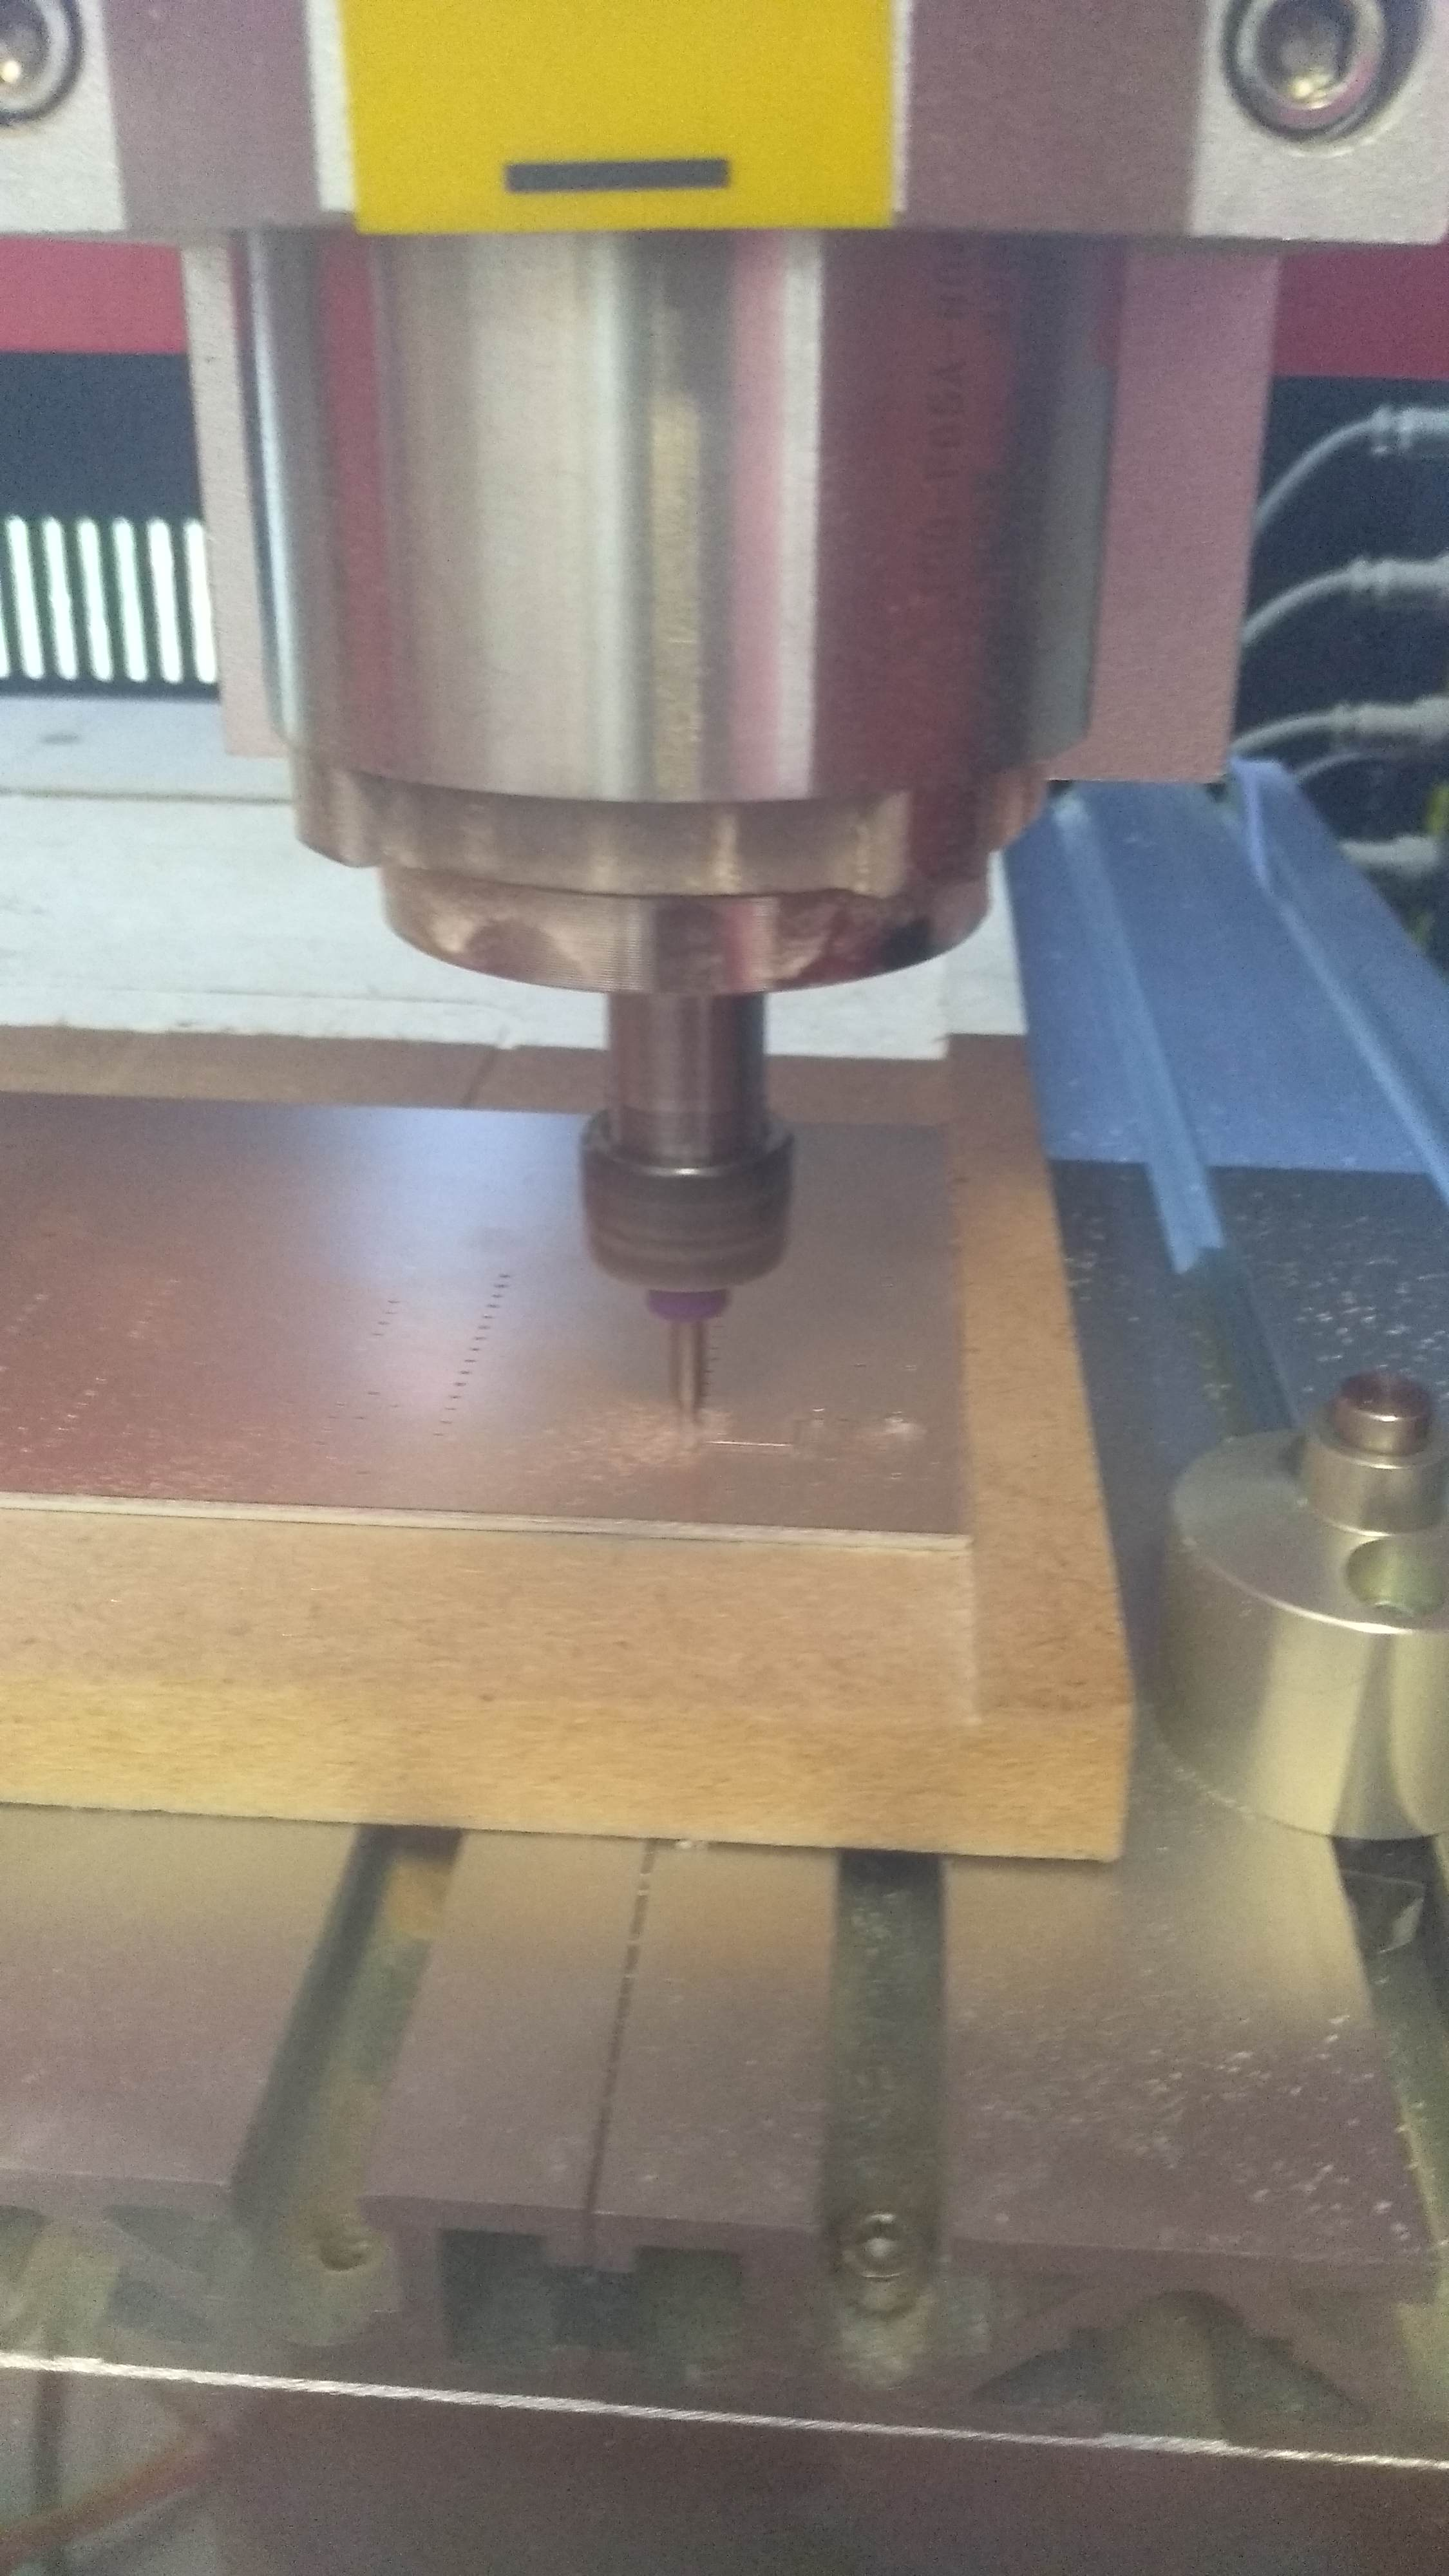
\includegraphics[width=0.2\textwidth]{img/CNCRouter.jpg}
	\label{img:RouterCNC}}
	\caption{Fabrication chez FabLab}
	\label{img:CampusFab}
\end{figure}

% \begin{figure}[!htb]
% \centering
% 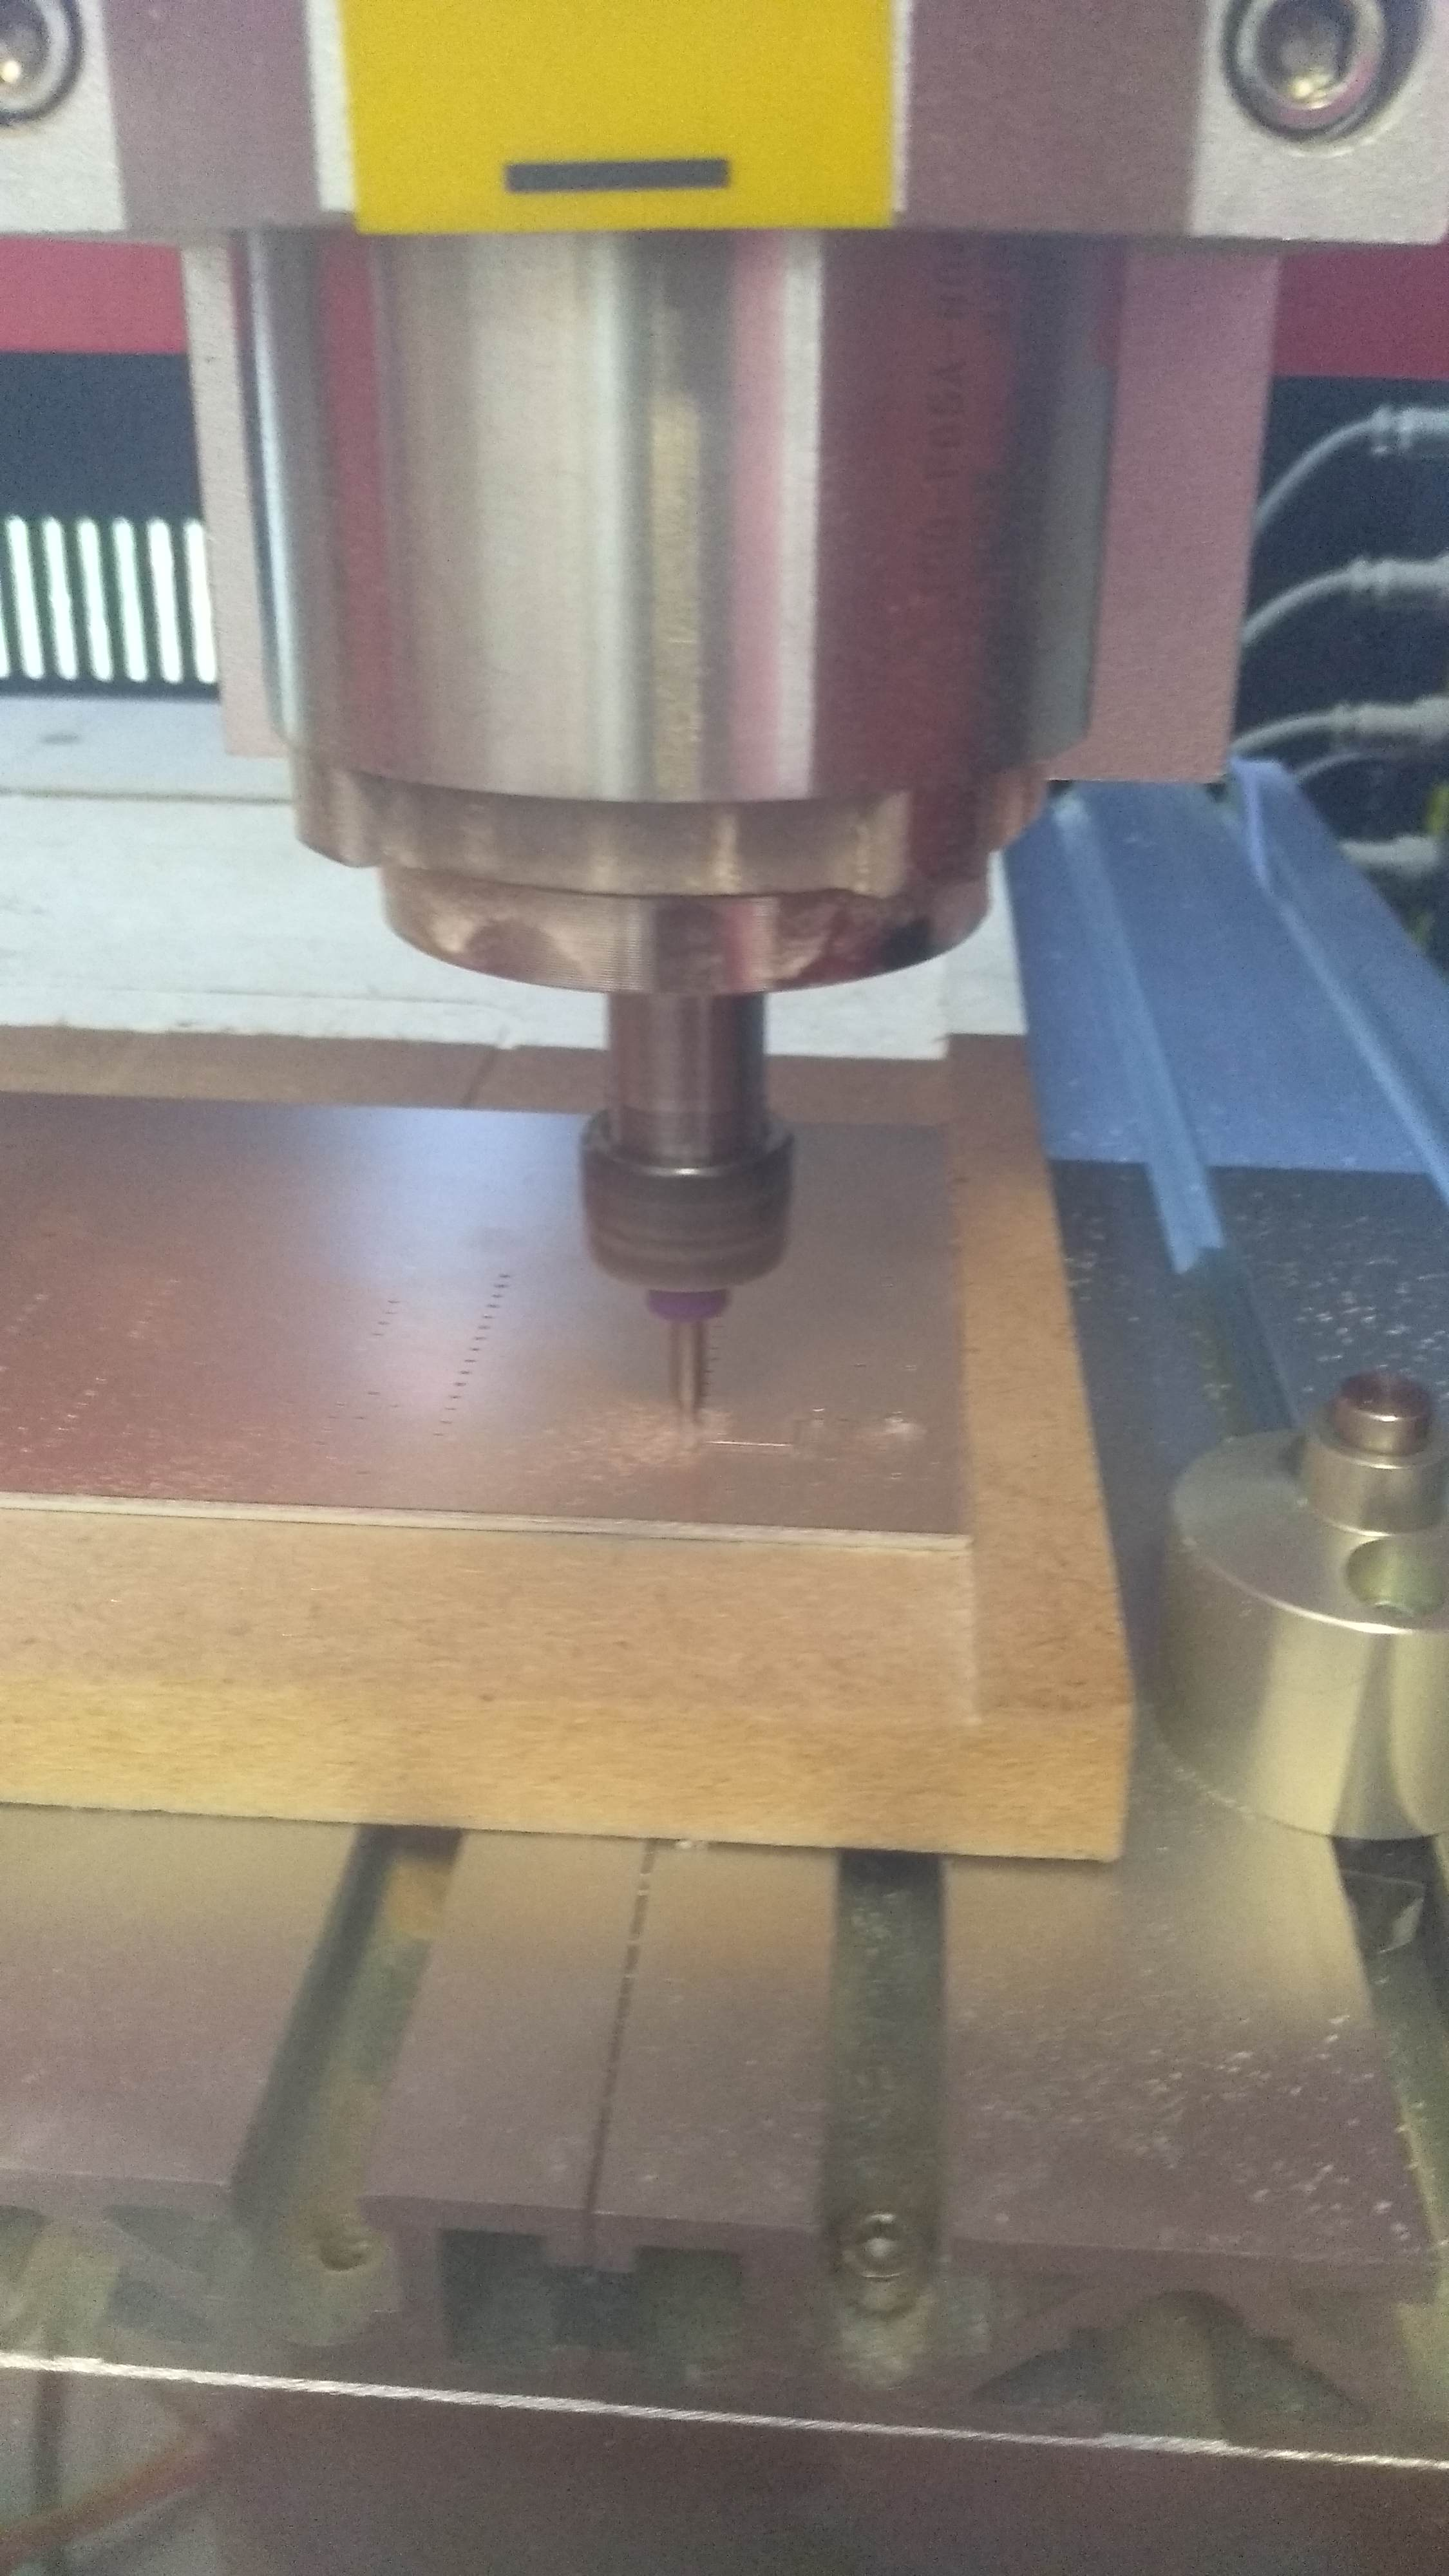
\includegraphics[width=0.2\textwidth]{img/CNCRouter.jpg}
% \caption{Machine CNC pour le routage des PCB}
% \label{img:RouterCNC}
% \end{figure}

% \begin{figure}[!htb]
% \centering
% \includegraphics[width=0.2\textwidth]{img/FlatCAM.png}
% \caption{Logiciel pour le routage des PCB}
% \label{img:flatcam}
% \end{figure}

% Luego de hacer los circuitos utilice la estacion de soldadura para montarlos componentes en la pcb.
\begin{par}
	Apr\`es avoir fabriqu\'e les PCB j'ai soud\'e les composants pour monter le
	circuit.
\end{par}

\begin{figure}[!htb]
\centering
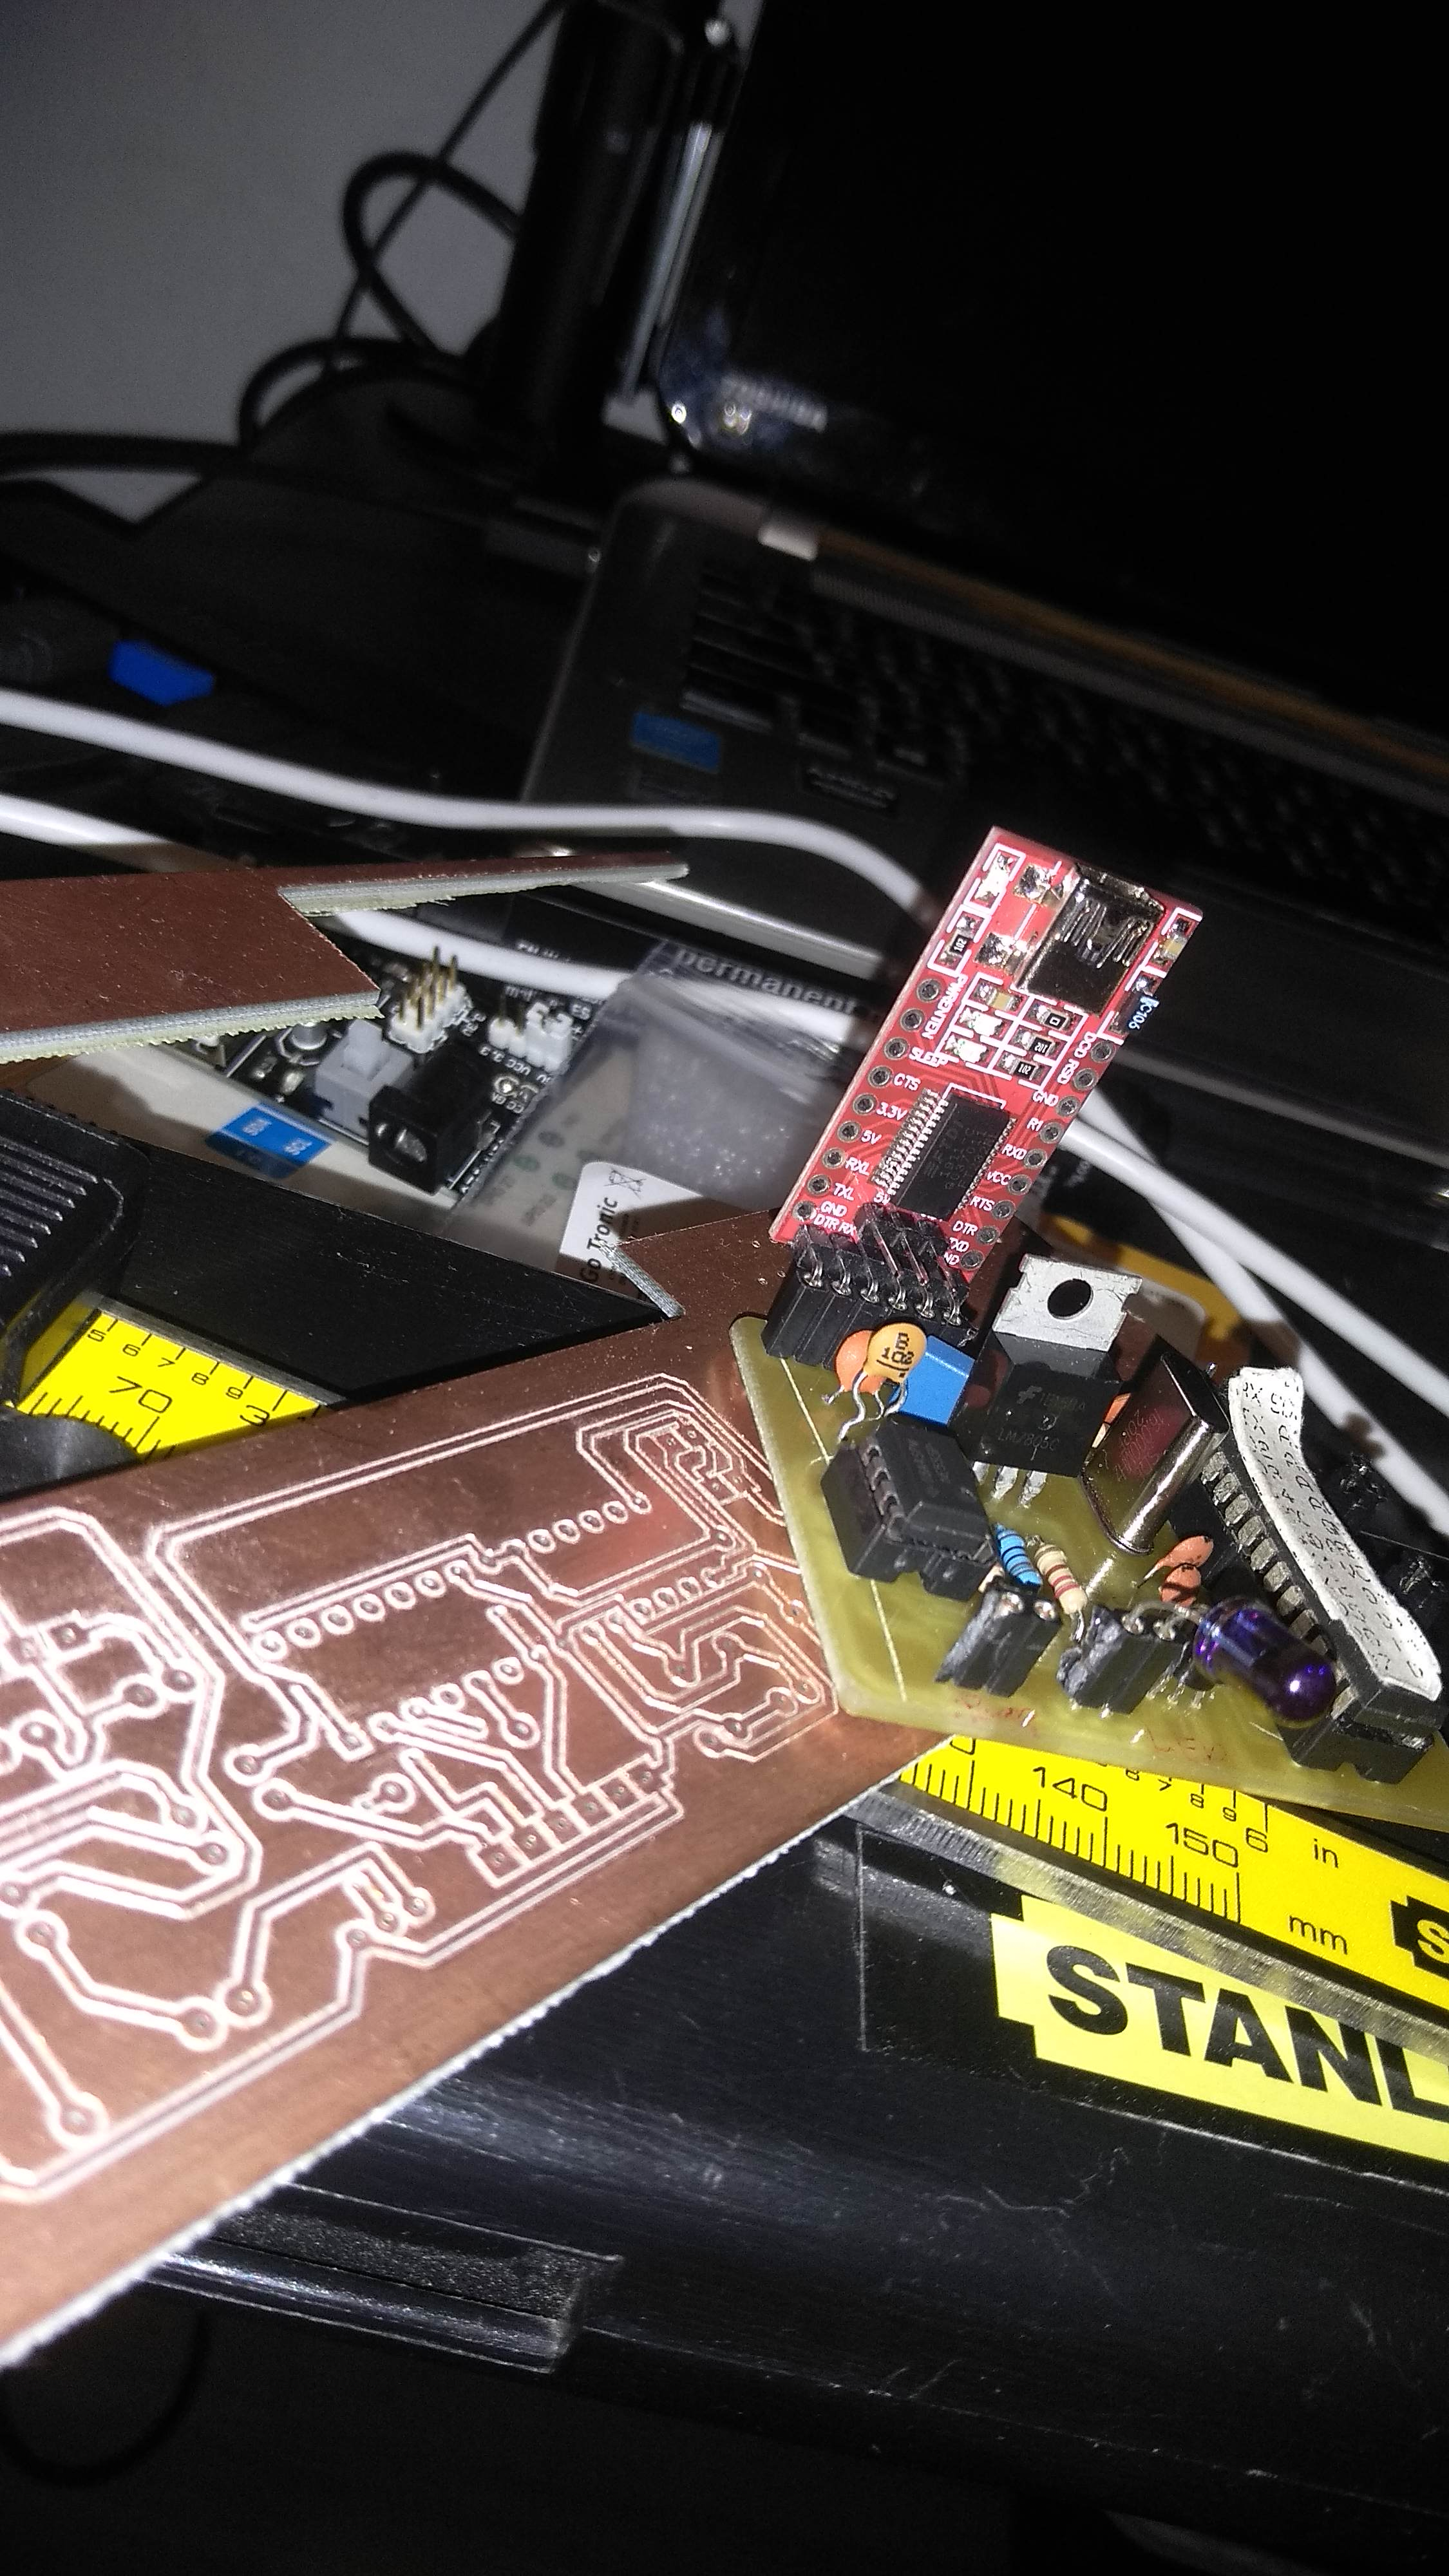
\includegraphics[width=0.2\textwidth]{img/CircuitosCNCed.jpg}
\caption{Des circuits apres le CNC Router}
\label{img:CircuitsCNCd}
\end{figure}
% La ultima herramienta que utilise fue la cortadora laser para hacer el soporte de las barieres IR y la nueva cajita del starting block (mas pequenha y tales)
Un autre outil que j'ai utilis\'e c'\'etait la decoupe laser pour decouper du plexiglass.
Dans l'image \ref{img:barriere} on peut voir.


\begin{figure}[!htb]
	\centering
	\subfigure[Decoupe Laser]{\includegraphics [height=2in]{img/CortadoraLaser.png}}
	\subfigure[Premiere essaye du Barriere IR]{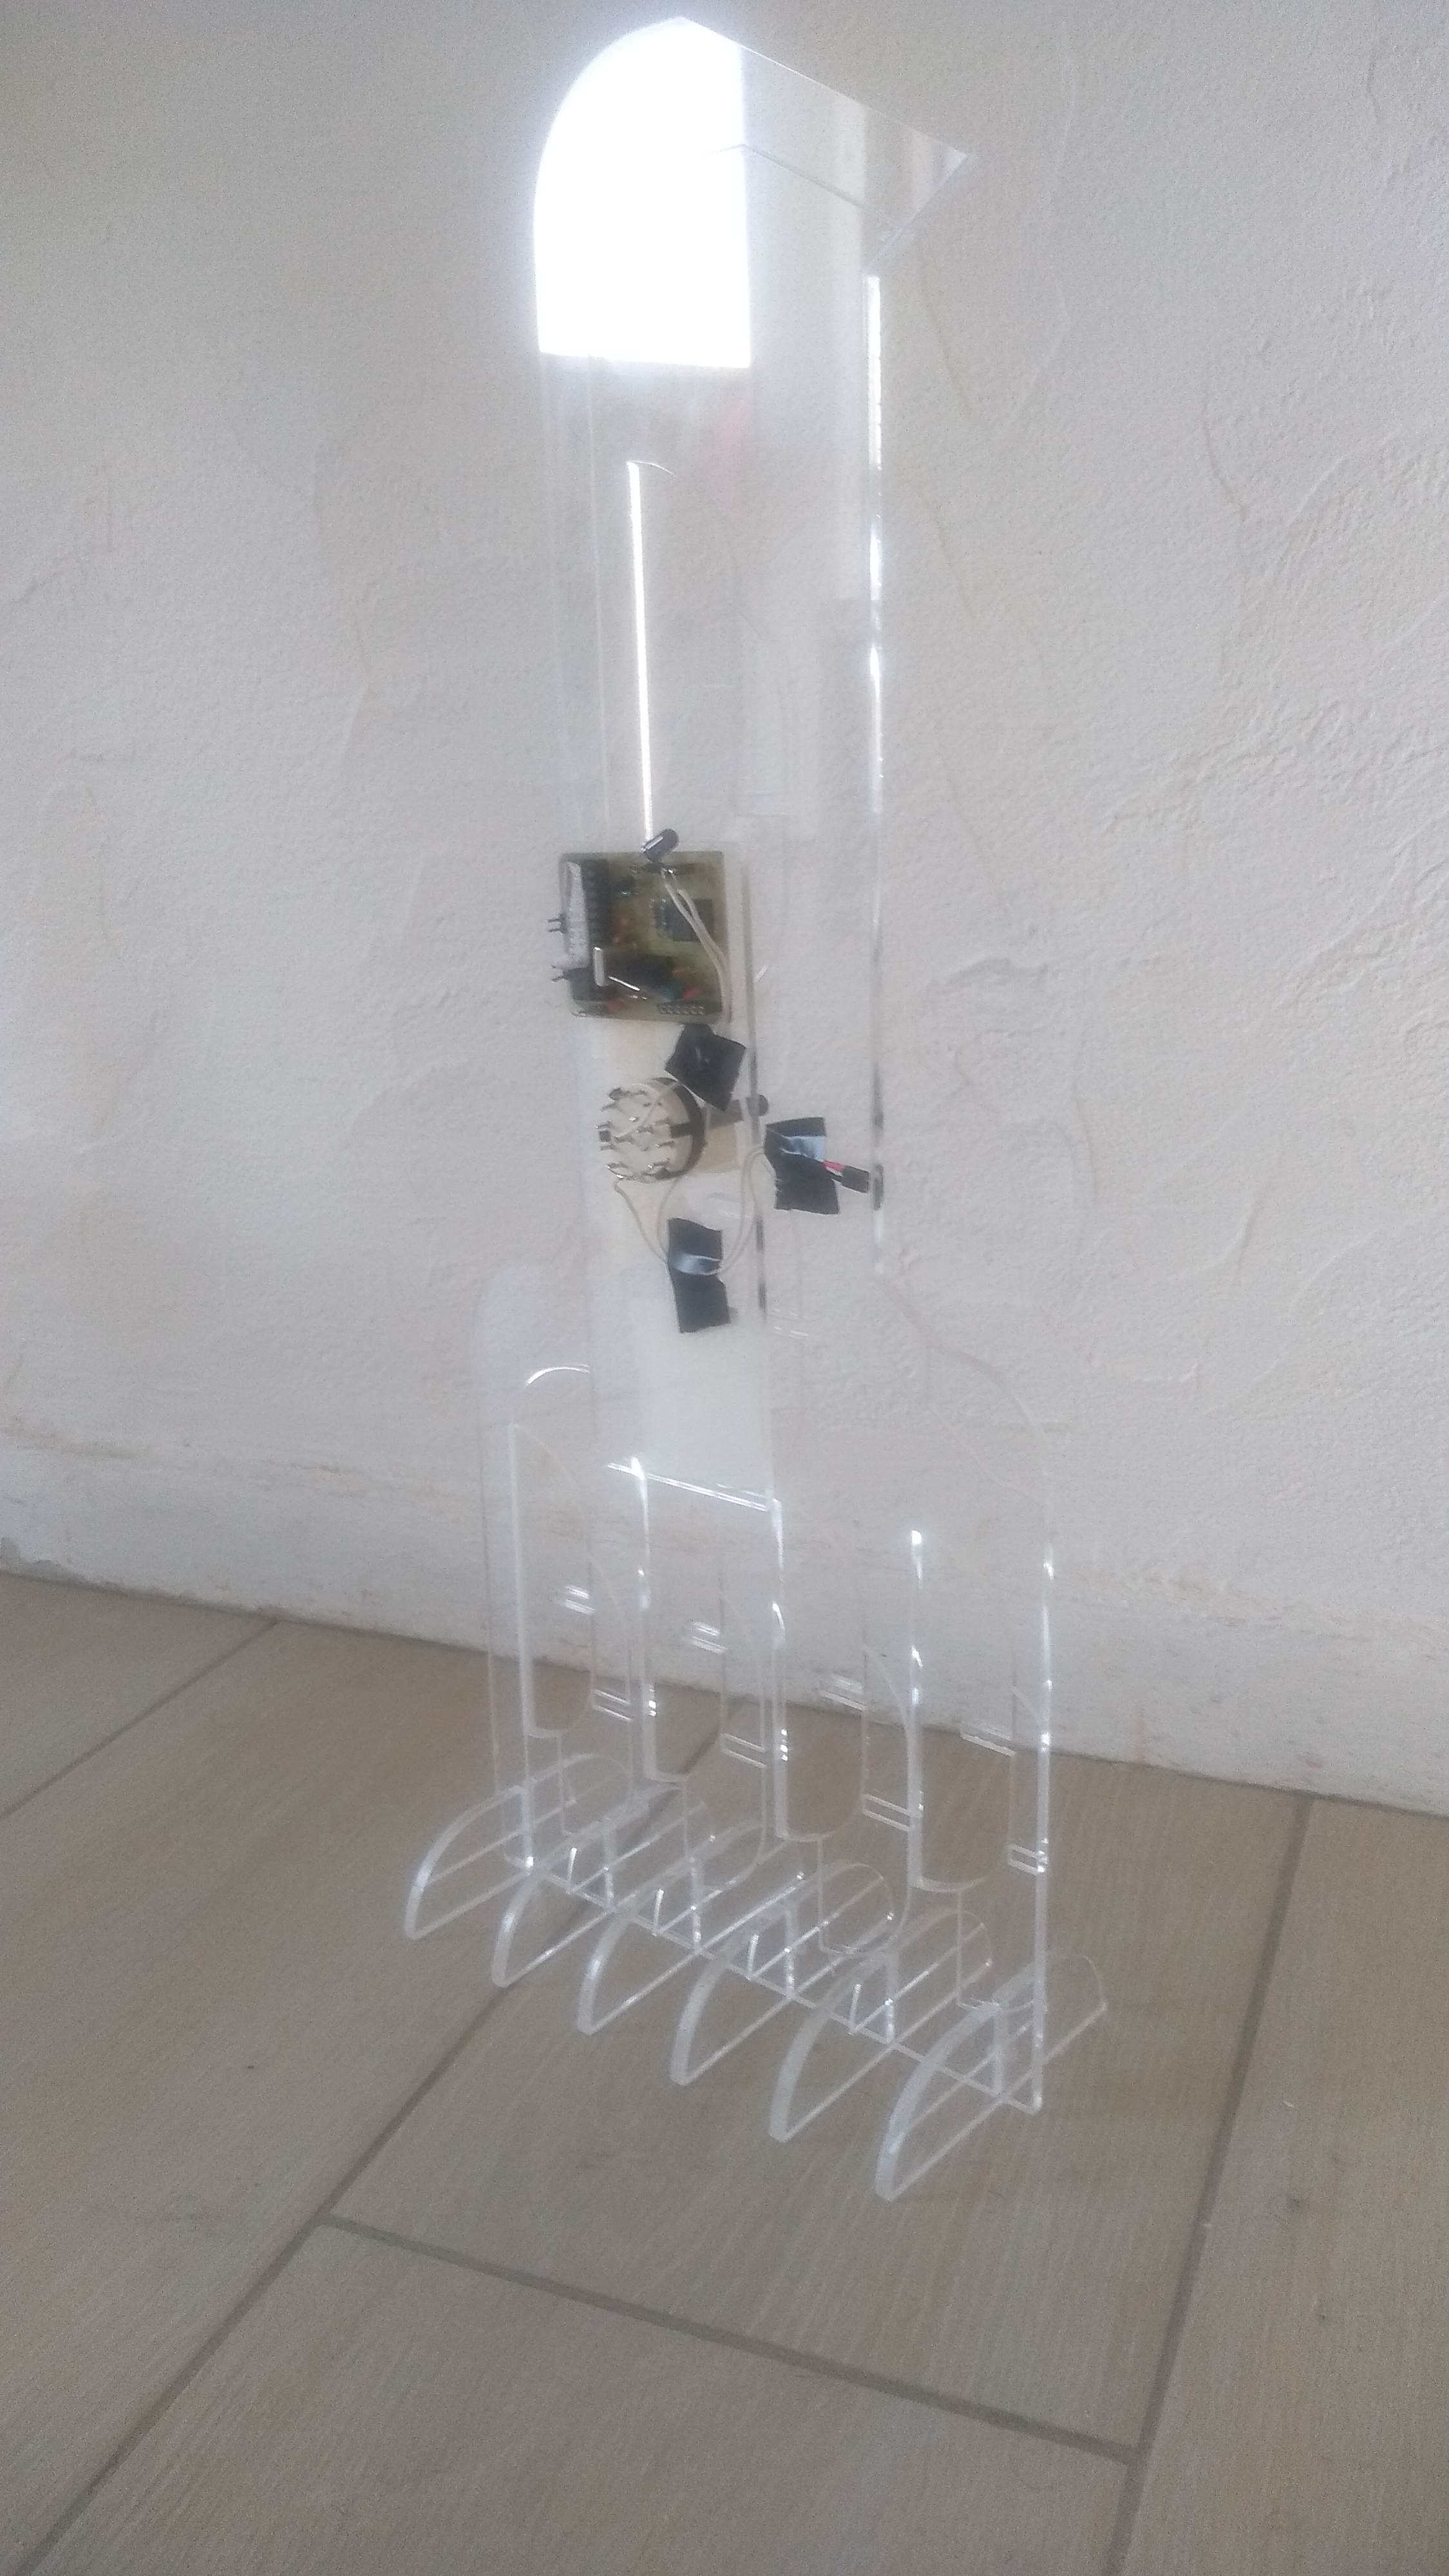
\includegraphics [height=2in]{img/BarriereIrV1.jpg}}
	\caption{Resultats de la decoupe laser}
	\label{img:barriere}
\end{figure}
% La impresora 3D tenia pensado usarla para hacer el temoin en PLA transparente y estuve imprimiento un cable chain para mejorar la robustez de los cables en el starting block.

% \begin{par}
% 	J'ai failli utiliser l'imprimante 3D pour faire 
% 	quelques pièces en fin du stage mais j'ai chop\'e
% 	le covid les dernieres semaines du juillet.
% \end{par}

\subsection{Github}
\begin{par}
	Ce projet etait un projet avec une grande 
	quantit\'e de programation dedans et j'ai choisi 
	git comme outil de gestion de versions. En plus,
	j'ai fait un repositoire sur Github pour avoir tout
	bien organis\'e et centralis\'e sur une seul 
	endroit.
\end{par}
% Al ser un proyecto donde mas de la mitad del trabajo es programacion es necesario tener un gestor de versiones para el cual utilise git. Ademas Github es excelente como herramienta de gestion compartida.

% Otra ventaja de github es que ofrece una pagina de wikis donde se puede dejar toda la documentacion por si alguien retoma el proyecto donde yo lo estoy dejando ahora mismo. Tambien tiene la seccion de gestion de proyectos que es parecida a slack donde pongo lo que voy haciendo poco a poco y el tutor de stage puede revisar mi trabajo poco a poco. 
\begin{par}
	Github nous offre une page de wikis pour la
	documentation du projet. Dans cette section j'ai 
	pens\'e laisser toutes les instructions pour les 
	developeurs et utilisateurs en general.
\end{par}
\begin{par}
	Sur Github nous trouverons aussi une section pour
	gerer des projets partag\'es de type slack ou
	trello. Sur l'image \ref{img:git:project} on peut
	le voir.
\end{par}

% La seccion de issues tambien es buenisima para el trabajo en grupo y si alguien a futuro tiene problemas con mi proyecto yo puedo ayudarlo a solucionar el problema.
\begin{par}
	La section issues de github permet de partager les
	probl\`emes avec autres developeurs, m\^eme si je
	ne fait plus part du projet.
\end{par}

\begin{figure}[!htb]
	\centering
	\subfigure[Repositoire sur github]{\includegraphics [height=2in]{img/Repo.png}
	\label{img:git:repo}}
	\subfigure[Outil de gestion de projets de github]{\includegraphics [height=2in]{img/GithubProject.png}
	\label{img:git:project}}
	\subfigure[Wikis sur github]{\includegraphics [width=2.7in]{img/GitWiki2.png}
	\label{img:git:wiki}}
	\caption{Images du repo}
	\label{img:git_all}
\end{figure}

%-------------------------- * Seccion de resultados * --------------------------------

\section{Results}
% Los resultados se vieron afectados por varios factores ajenos al desarrollo del proyecto como mi rattrapage a mitad de junio, varias pcb que vinieron malas y faltando dos semanas para terminar el stage me dio covid y cuando pude salir el fablab estaba cerrado y solo me faltaba terminar de fabricar las piezas del temoin. Para colmo se quemaron 2 step up y no pude nisiquiera pude soldar los temoin (y habia uno que tenia unos vias que no hacian conexion, maldita sea). A pesar de todo eso pude avanzar mucho en otras cosas.
\begin{par}
	Le projet a eu un developement lent dû à ma manque
	d'experience mais en géneral j'ai bien ger\'e le temp.
	Les prob\`emes que j'ai eu ont \'et\'e \`a cause 
	des cartes electroniques d\'efectueuses.
\end{par}
\begin{par}
	Pour la partie software, j'avais d\'ej\`a 
	travaill\'e avec python et le framework de l'interface
	ce qui m'a rendu un peu facile le travail de 
	programation.
\end{par}
\begin{par}
	Comme dernier souci j'ai eu le covid en fin du 
	stage et je n'ai pas pu finir quelques choses chez
	CampusFab parce que j'ai dû me confiner. Ces jours de
	confinement j'ai avanc\'e la programation d'un
	base de donn\'ees plus robuste et pr\^ete \`a 
	utiliser m\^eme sans les prototypes.
\end{par}

%-------------------

\subsection{Dock multiplataforme}
% La raspberry como dock multifuncional es le mejor avance que hice ya que ahora tiene una base de datos que permite ingresar atletas, coachs y llevar un historal de todas las sesiones de entrenamiento. Ademas se conecta directamente al starting block y permite ver su estado de bateria. 
% Tambien permite actualizar la interfaz directamente desde github, lo que permitiria venderlo como producto y actualizarlo con el pasar del tiempo.
% Toda la informacion guardada es ademas exportable por si se quiere hacer un tratamiento de datos externo.

\begin{par}
	Le dock multiplataforme est 
	l'avancement le plus remarquable de mon stage. Il 
	a une base de donn\'ees complete avec l'information
	de chaque coach et athlete. Sur l'image \ref{img:gui_all}
	on peut voir la liste de seances et le graph g\'ener\'e
	par le dock.
	Il se connecte avec 
	un smartphone, tablette ou m\^eme un ordinateur via
	WiFi direct pour manipuler et voir les donn\'ees.
	Sur l'image \ref{img:gui:landing-page} on peut voir
	la premier page de l'interface vu depuis un 
	ordinateur.
\end{par}

\begin{figure}[!htb]
	\centering
	\includegraphics[width=0.4\textwidth]{img/LandingPage.png}
	\caption{Page d'accueil}
	\label{img:gui:landing-page}
\end{figure}

\begin{figure}[!htb]
	\centering
	\subfigure[Seance Detaill\'e]{\includegraphics [height=2in]{img/SessionDetail}
	\label{img:gui:session-detail}}
	\subfigure[Liste de seances stock\'ees]{\includegraphics [height=2in]{img/SessionList}
	\label{img:gui:session-list}}
	\caption{Base de donn\'ees.}
	\label{img:gui_all}
\end{figure}

% \begin{par}
% 	En plus, elle peut \^etre mise \`a jour avec github
% 	et donc si on change des choses sur l'interface au 
% 	niveau du graphisme ou de manipulation de don\'ees
% 	de l'autre c\^ot\'e du monde, on peut voir ces 
% 	changements sur la raspi.
% \end{par}
\begin{par}
	Malheureusement la partie de hardware pour connecter
	les temoins et extraire les données n'a pas pu être
	fini à cause du covid parce que je n'ai pas pu aller
	chez CampusFab pour finir la fabrication.
	% lastimosamente la parte de los temoins no la pude
	% terminar por el covid y porque la mayoria de las 
	% tarjetas electronicas del servicio de la fac vinieron
	% con defectos.
\end{par}

\subsection*{Travail \`a futur}
% Como mejora esta meterle una bateria y que esta cargue los temoins. Mostrar tambien la carga del propio aparato. y terminar la parte que se conecta con el temoin, la cual esta testeada con datos simulados que funcionan bien.
% Otra mejora que tengo pensado ponerle es una opcion que permita un calibrage automatico de los sensores de fuerza para no tener que desarmar el dispositivo cada vez que se descalibre.
\begin{par}
	La premier chose à ameliorer est avoir une baterie qui charge
	les temoins et qui donne une bonne autonomie au dock et finir la
	partie de conexion pour les temoins.
	% Meterle una bateria para que cargue los temoins, hacerle la conexion para que se connecte con los temoins y 
	% de paso que los cargue. Hacerle pruebas para calcular la autonomia de la bateria y la vaina.
\end{par}
% \begin{par}

% 	Algo que me gustaria agregarle es una parte de calibrage automatico de los sensores de presion
% 	en el starting block
% \end{par}

%-------------------

\subsection{Startingblock 2.0}
% El mayo cambio en el starting block en terminos de harwdware es su tamanho mas reducido y el uso de una bateria de ion de litio recargable directamente desde la cajita. Segun las pruebas de rendimiento el dispositivo consume aproximadamente unos 100mA de corriente de forma constante con pequenhos picos de corriente de 200mA por lo cual se puede estimar la duracion de la bateria. (aqui pones fotos del videito que grabaste)
\begin{par}
	La boîte electronique du starting block est plus 
	petite et plus efficace d'un point de vue energetique.
	Maintenant il a un chargeur interne avec une conexion
	mirco-usb qui permet le charger avec un chargeur
	commercial. Image \ref{img:sb:complete}
\end{par}

\begin{figure}[!htb]
	\centering
	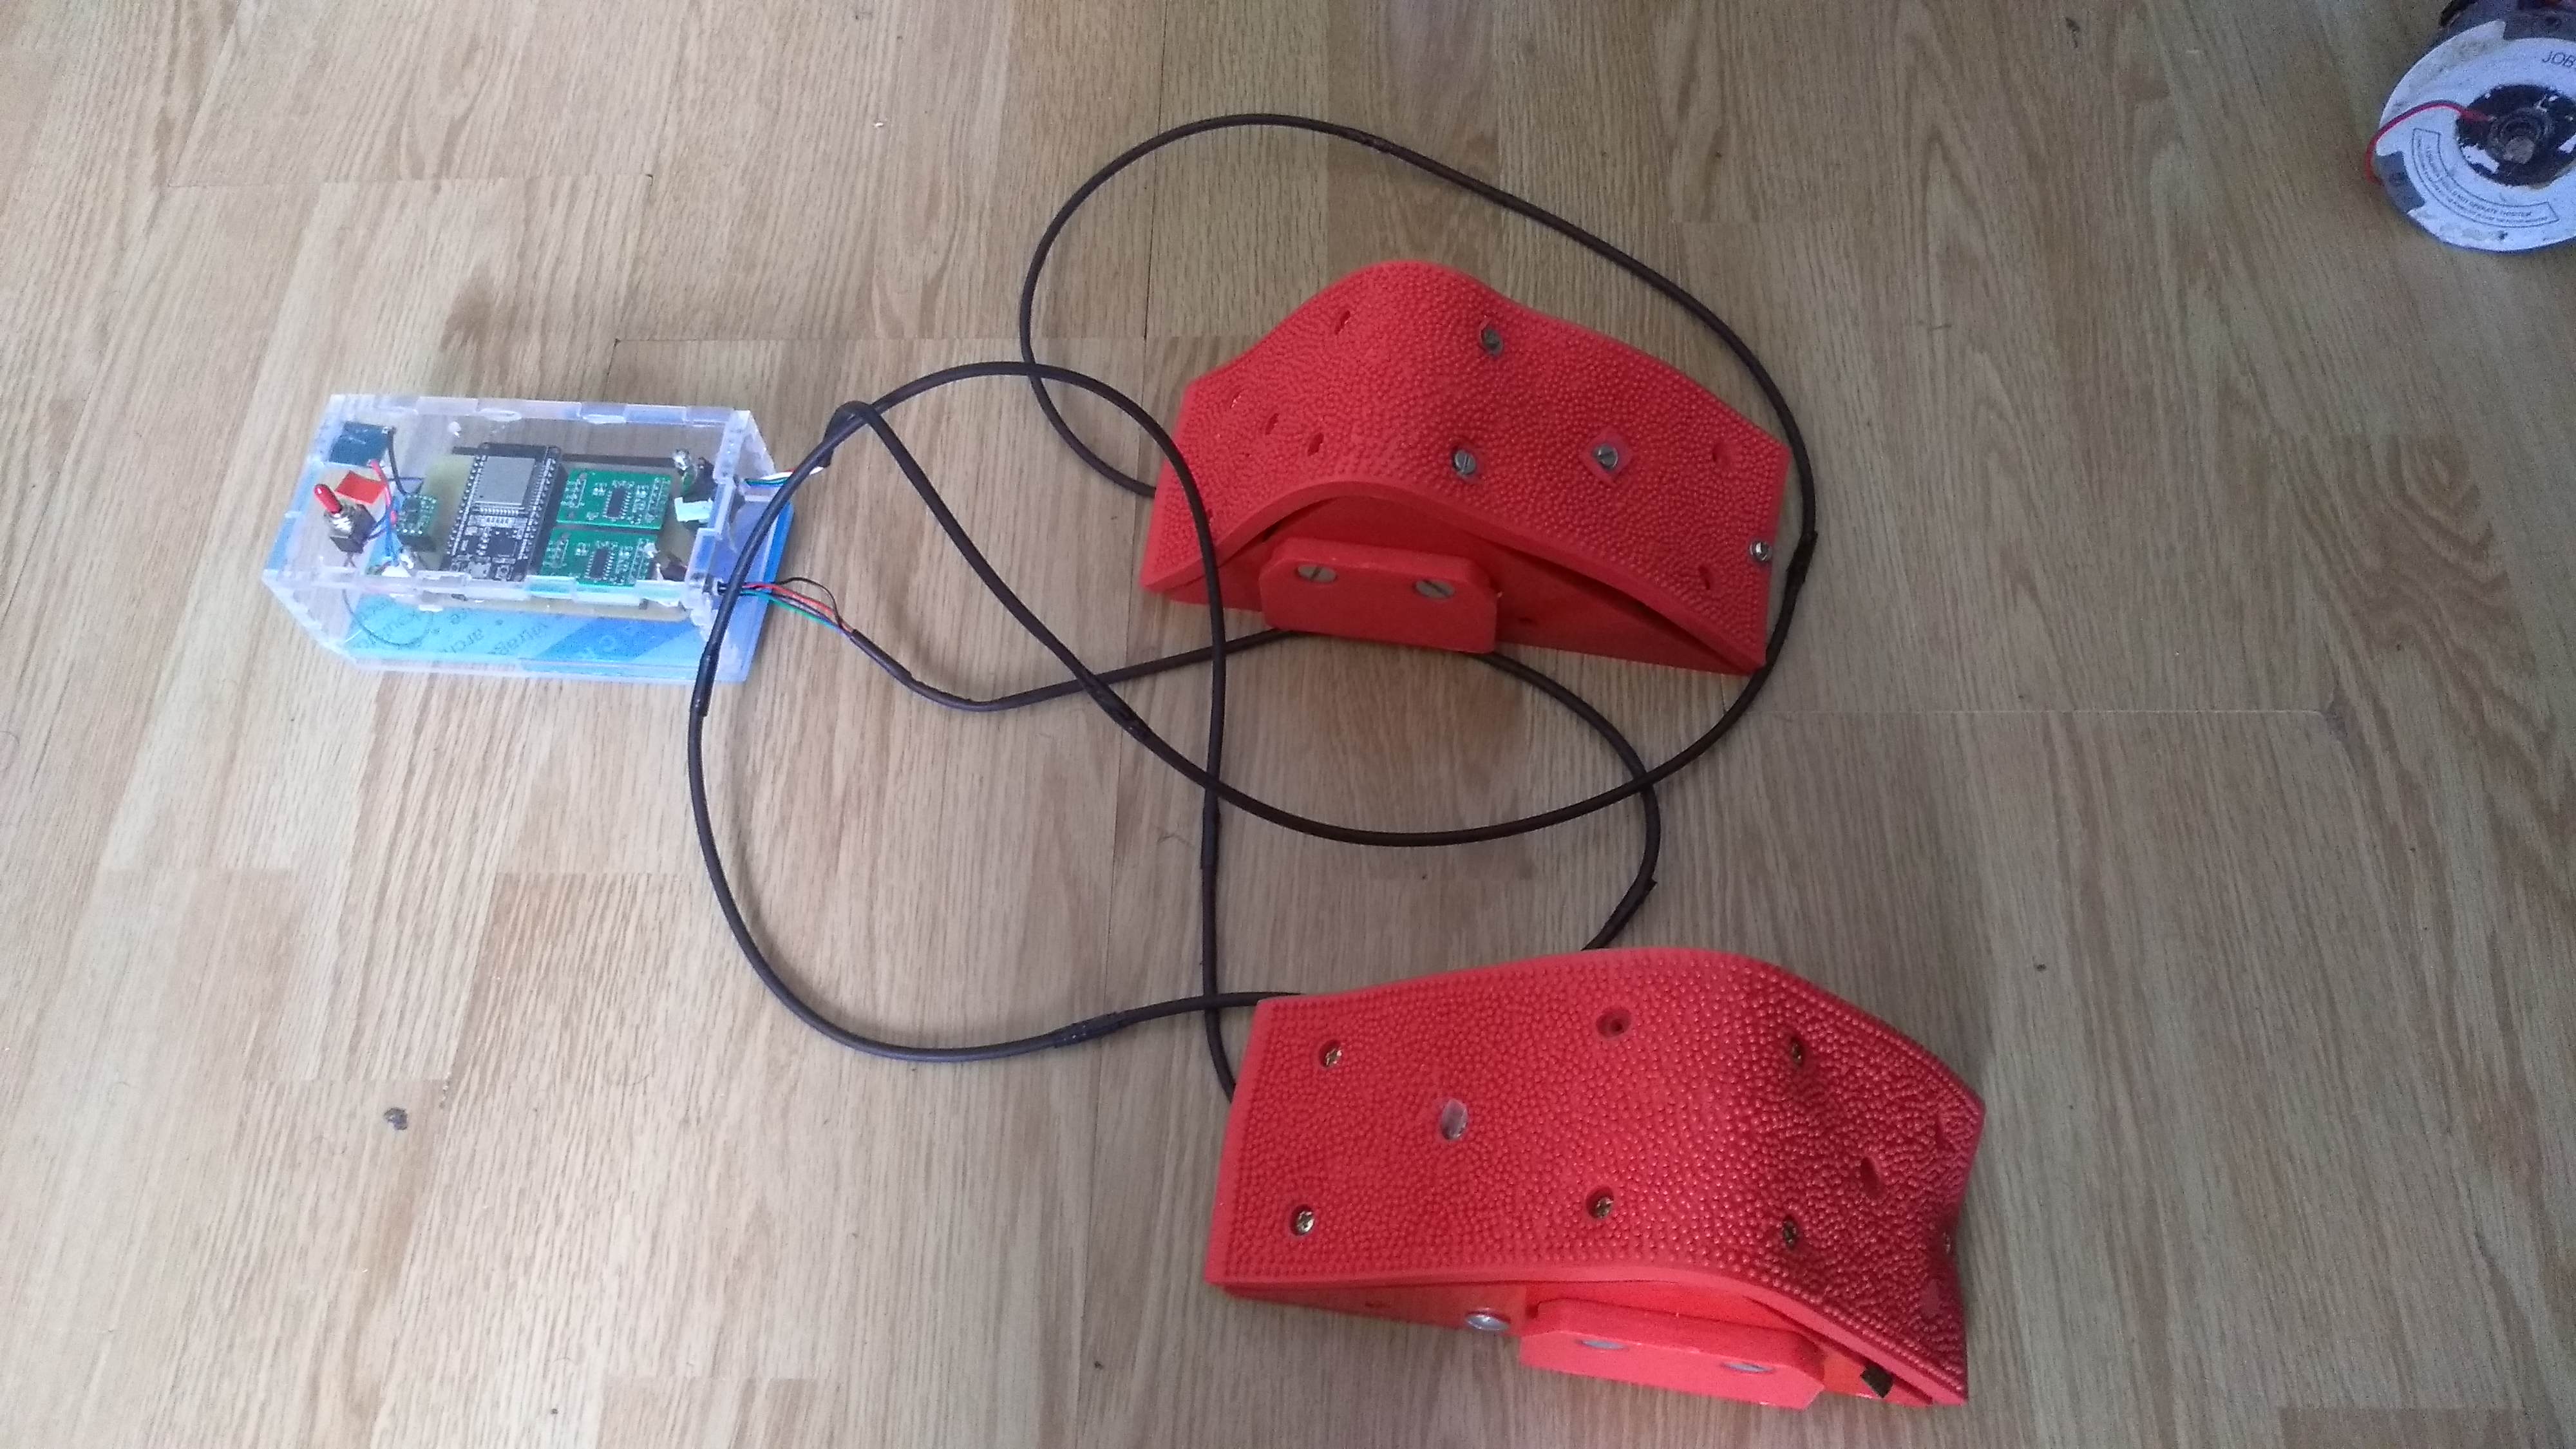
\includegraphics[width=0.5\textwidth]{img/StartingBlockCompleto.jpg}
	\caption{Starting Block}
	\label{img:sb:complete}
\end{figure}

\subsection*{Travail Futur}
\begin{par}
	Ajouter un script de calibration lanc\'e par le dock. 
	Ameliorer la conception pour un possible depanage et
	un condensateur qui aide
	la batterie dans les piques de courant.
\end{par}
% Agregarle a la programacion el programa de calibracion (el cual ya viene listo en la libreria de los amplificadores) que se haga directamente desde la interfaz grafica.

% Otra cosa que no tuve en cuenta es el disenho que favorezca un depanage. Actualmente es muy complicado desarmar todo para revisar si algo falla, eso fue un error de disenho que no tuve en cuenta.
% Una ultima mejora es agregarle un capacitor que ayude a la bateria en los picos de corriente para aumentar la vida util de la bateria.

%-------------------

\subsection{Temoin et Course de relais}
% Los temoin y las barrieres IR tuvieron una mejora sustancial en terminos de usabilidad y componentes. Lastima que las pcb del protipo final vinieron con fallas y no se pudo armar un dispositivo final, ademas que habian unos step up que se quemaron y solo me quedaba uno y lo use para el starting block que ya estaba armado para tener una cosa que sirviera. Ademas de todo esto, la imposibilidad de ir al fablab la ultima semana me limito mucho porque tuve covid y aja eso me cago la vida.
\begin{par}
	Les temoins et les barrieres IR ont eu une upgrade 
	enorme avec les nouveaux composants. Fâcheusement
	les cartes electroniques faites par l'université
	avaient des defauts de fabrication et quelques
	composants de puissance ont br\^ul\'e quand le service
	de commandes de l'université est allé en congés.
\end{par}
\subsection*{Travail Futur}
\begin{par}
	Il me manque monter et tester les prototypes, mais j'ai déjà pensé
	à faire une conception un peut plus adapté au depanade rapide.
\end{par}
% Basicamente falta armarlos y probarlos, ahi falle pero me perjudico la situacion sanitaria ya que esta semana tenia pensado hacer esas cosas.

%-------------------

\subsection{Documentacion del proyecto}

\begin{par}
	La documentation du projet se trouve sur la page de wikis du repo
	sur github. Elle a des sections pour les developeurs futurs et pour
	les utilisateurs à futur
\end{par}
\begin{par}
	Pour la documentation des codes en C et C++ j'ai utilisé d'oxygen.
\end{par}
% La documentacion actual es la de la version del poryecto TER y me falta agregarle todas las cosas que desarrolle hasta este momento. Viendo que utilise un framework web y que no todo el mundo sera capaz de utilizar este framework intente factorizar las funciones al maximo para que cualquier pueda modificar las funciones que hacen las cosas importantes sin tener que meterse directamente con el framework.
% Para documentar tambien utilise doxygen que genero un archivo pdf con la explicacion de todas las funciones en C.

\begin{figure}[!htb]
	\centering
	\includegraphics[width=0.5\textwidth]{img/GitWiki.png}
	\caption{Wikis du Github}
	\label{img:git:wikis1}
\end{figure}

\subsection*{Travail Futur}
\begin{par}
	Vu que j'utilise Django, un framework optimisé pour la web, j'aimerais 
	documenter le fonctionement du framework pour les developeurs qui ne
	sont pas habitués a ce type de fonctionement.
\end{par}
% Me encantaria documentar todo el framework de django pero es un trabajo largo y duro, asi que lo dejo como trabajo futuro.

%\begin{figure}[!htb]
%\centering
%\includegraphics[width=0.2\textwidth]{images/ubication-sipi.png}
%\caption{Location du village Sipí \cite{sipi:ubicacion}}
%\label{img:sipi:ubicacion}
%\end{figure}

% Plantilla para colocar muchas imagenes con un multiplot
%\begin{figure}[!htb]
%\centering
%\subfigure[Photo trouv\'e sur Facebook]{\includegraphics %[height=2in]{images/image18.png}
%\label{img:sipi-urbana}}
%\subfigure[Photo prise par la mairie de Sip\'i ]{\includegraphics %[height=2in]{images/alcaldia-sipi.jpg}
%\label{img:sipi-urbana2}}
%\subfigure[Photo pris par le quotidien Colombien \textit{CNC Noticias}]{\includegraphics %[width=2.7in]{images/image39.png}
%\label{img:sipi-urbana3}}
%\caption{Images de Sip\'i}
%\end{figure}
%Sur la Figure \ref{img:sipi:boats} on peut voir les bateaux transportant des personnes et des biens.



%Para citar la bibliografia haces \cite{Photovoltaic}
%Para referenciar las imagenes haces lo sgte \ref{fig:schema}


\section{Conclusion}
% Este stage fue muy interesante y aprendi muchas cosas como gestionar un proyecto, usar diferentes logiciels para plantear las cosas e incluso utilise plantuml para planear las cosas pero no funciono del todo, cagada eso. Aprendi mucho y estuvo bueno todo mientras duro.
\begin{par}
	Ce stage a \'et\'e tr\`es interessant parce que
	c'est la premier fois que je fais un projet 
	financ\'e par une universit\'e, d'habitude nous
	avons limitations technologiques en tant qu'\'etudiants
	mais dans ce projet j'ai eu un budget plus genereux
	et cela m'a fait rechercher les meilleurs composants
	pour le projet.
\end{par}
\begin{par}
	% C'etait interesant aussi faire la conception,
	% fabrication et montage de chaque un des appareils
	% du projet.
	J'ai bien aimé faire partie du conception, fabrication et
	montage de chaque appareil.
\end{par}
\begin{par}
	Je vais suivre ce projet en tant que stagiaire pour
	l'ann\'ee prochaine et faire une alternance (si possible)
	pour faire toutes les ameliorations propos\'es precedement.
\end{par}

%debes hacer esto para meter archivos de otro lado
%\input{sub_files/Calcul_puissance}
%\label{anexe:calcul-puissance}
%-------------------

%Para meter un pdf haces lo sgte 
%\includepdf{images/Velocidad-Maxima-Energia_13}
%\label{pdf:vent_vitesse_max}
%-------------------

% \begin{figure}
%     \centering
%     \includegraphics[height=\textheight]{Anexes/RadiacionSolar13 (1).pdf}
%     \caption{Caption}
%     \label{fig:radiacion}
% \end{figure}


% Plantilla para colocar muchas imagenes con un multiplot
%\begin{figure}[!htb]
%\centering
%\subfigure[]{\includegraphics [width=2.5in]{lab_2_vision_15.png}}
%\subfigure[]{\includegraphics [width=2.5in]{lab_2_vision_16.png}}
%\subfigure[]{\includegraphics [width=2.5in]{lab_2_vision_17.png}}
%\caption{Paleta de colores}
%\end{figure}

% Plantilla para poner una imagen cualquiera
%\begin{figure}[!htb]
%\centering
%
%\caption{Histograma de la imagen}
%\end{figure}

%\bibliography{Biblio}

\end{document}
